%%%%%%%%%%%%%%%%%%%%%%%%%%%%%%%%%%%%%%%%%
% a0poster Portrait Poster
% LaTeX Template
% Version 1.0 (22/06/13)
%
% The a0poster class was created by:
% Gerlinde Kettl and Matthias Weiser (tex@kettl.de)
% 
% This template has been downloaded from:
% http://www.LaTeXTemplates.com
%
% License:
% CC BY-NC-SA 3.0 (http://creativecommons.org/licenses/by-nc-sa/3.0/)
%
%%%%%%%%%%%%%%%%%%%%%%%%%%%%%%%%%%%%%%%%%

%----------------------------------------------------------------------------------------
%  PACKAGES AND OTHER DOCUMENT CONFIGURATIONS
%----------------------------------------------------------------------------------------

\documentclass[a0,portrait]{a0poster}\usepackage[]{graphicx}\usepackage[]{color}
%% maxwidth is the original width if it is less than linewidth
%% otherwise use linewidth (to make sure the graphics do not exceed the margin)
\makeatletter
\def\maxwidth{ %
  \ifdim\Gin@nat@width>\linewidth
    \linewidth
  \else
    \Gin@nat@width
  \fi
}
\makeatother

\definecolor{fgcolor}{rgb}{0.345, 0.345, 0.345}
\newcommand{\hlnum}[1]{\textcolor[rgb]{0.686,0.059,0.569}{#1}}%
\newcommand{\hlstr}[1]{\textcolor[rgb]{0.192,0.494,0.8}{#1}}%
\newcommand{\hlcom}[1]{\textcolor[rgb]{0.678,0.584,0.686}{\textit{#1}}}%
\newcommand{\hlopt}[1]{\textcolor[rgb]{0,0,0}{#1}}%
\newcommand{\hlstd}[1]{\textcolor[rgb]{0.345,0.345,0.345}{#1}}%
\newcommand{\hlkwa}[1]{\textcolor[rgb]{0.161,0.373,0.58}{\textbf{#1}}}%
\newcommand{\hlkwb}[1]{\textcolor[rgb]{0.69,0.353,0.396}{#1}}%
\newcommand{\hlkwc}[1]{\textcolor[rgb]{0.333,0.667,0.333}{#1}}%
\newcommand{\hlkwd}[1]{\textcolor[rgb]{0.737,0.353,0.396}{\textbf{#1}}}%

\usepackage{framed}
\makeatletter
\newenvironment{kframe}{%
 \def\at@end@of@kframe{}%
 \ifinner\ifhmode%
  \def\at@end@of@kframe{\end{minipage}}%
  \begin{minipage}{\columnwidth}%
 \fi\fi%
 \def\FrameCommand##1{\hskip\@totalleftmargin \hskip-\fboxsep
 \colorbox{shadecolor}{##1}\hskip-\fboxsep
     % There is no \\@totalrightmargin, so:
     \hskip-\linewidth \hskip-\@totalleftmargin \hskip\columnwidth}%
 \MakeFramed {\advance\hsize-\width
   \@totalleftmargin\z@ \linewidth\hsize
   \@setminipage}}%
 {\par\unskip\endMakeFramed%
 \at@end@of@kframe}
\def\verbatim{\small\@verbatim \frenchspacing\@vobeyspaces \@xverbatim}
\makeatother

\definecolor{shadecolor}{rgb}{.97, .97, .97}
\definecolor{messagecolor}{rgb}{0, 0, 0}
\definecolor{warningcolor}{rgb}{1, 0, 1}
\definecolor{errorcolor}{rgb}{1, 0, 0}
\newenvironment{knitrout}{}{} % an empty environment to be redefined in TeX

\usepackage{alltt}
\usepackage[utf8]{inputenc}

\usepackage{multicol} % This is so we can have multiple columns of text side-by-side
\columnsep=100pt % This is the amount of white space between the columns in the poster
\columnseprule=1pt % This is the thickness of the black line between the columns in the poster

\usepackage[svgnames]{xcolor} % Specify colors by their 'svgnames', for a full list of all colors available see here: http://www.latextemplates.com/svgnames-colors

\usepackage{times} % Use the times font
%\usepackage{palatino} % Uncomment to use the Palatino font

\usepackage{graphicx} % Required for including images
\graphicspath{{figs/}} % Location of the graphics files
\usepackage{booktabs} % Top and bottom rules for table
\usepackage[font=small,labelfont=bf]{caption} % Required for specifying captions to tables and figures
\usepackage{wrapfig} % Allows wrapping text around tables and figures

%bib
\usepackage{natbib}

% Math
\usepackage{amsfonts, amsmath, amsthm, amssymb} % For math fonts, symbols and environments
\DeclareMathOperator{\tr}{tr}
\DeclareMathOperator{\diag}{diag}


\newcommand{\mysec}[1]{\color{Black}\section*{#1}\color{DarkSlateGray}}
\IfFileExists{upquote.sty}{\usepackage{upquote}}{}
\newcommand{\code}[1]{\texttt{#1}}
\newcommand{\inputR}[1]{\input{#1}}
\usepackage{hyperref}

\providecommand{\tightlist}{\setlength{\itemsep}{0pt}\setlength{\parskip}{0pt}}

% Code highlighting
\usepackage{color}
\usepackage{fancyvrb}
\newcommand{\VerbBar}{|}
\newcommand{\VERB}{\Verb[commandchars=\\\{\}]}
\DefineVerbatimEnvironment{Highlighting}{Verbatim}{commandchars=\\\{\}}
% Add ',fontsize=\small' for more characters per line
\usepackage{framed}
\definecolor{shadecolor}{RGB}{248,248,248}
\newenvironment{Shaded}{\begin{snugshade}}{\end{snugshade}}
\newcommand{\KeywordTok}[1]{\textcolor[rgb]{0.13,0.29,0.53}{\textbf{{#1}}}}
\newcommand{\DataTypeTok}[1]{\textcolor[rgb]{0.13,0.29,0.53}{{#1}}}
\newcommand{\DecValTok}[1]{\textcolor[rgb]{0.00,0.00,0.81}{{#1}}}
\newcommand{\BaseNTok}[1]{\textcolor[rgb]{0.00,0.00,0.81}{{#1}}}
\newcommand{\FloatTok}[1]{\textcolor[rgb]{0.00,0.00,0.81}{{#1}}}
\newcommand{\CharTok}[1]{\textcolor[rgb]{0.31,0.60,0.02}{{#1}}}
\newcommand{\StringTok}[1]{\textcolor[rgb]{0.31,0.60,0.02}{{#1}}}
\newcommand{\CommentTok}[1]{\textcolor[rgb]{0.56,0.35,0.01}{\textit{{#1}}}}
\newcommand{\OtherTok}[1]{\textcolor[rgb]{0.56,0.35,0.01}{{#1}}}
\newcommand{\AlertTok}[1]{\textcolor[rgb]{0.94,0.16,0.16}{{#1}}}
\newcommand{\FunctionTok}[1]{\textcolor[rgb]{0.00,0.00,0.00}{{#1}}}
\newcommand{\RegionMarkerTok}[1]{{#1}}
\newcommand{\ErrorTok}[1]{\textbf{{#1}}}
\newcommand{\NormalTok}[1]{{#1}}



\begin{document}

%----------------------------------------------------------------------------------------
%  POSTER HEADER 
%----------------------------------------------------------------------------------------

% The header is divided into two boxes:
% The first is 75% wide and houses the title, subtitle, names, university/organization and contact information
% The second is 25% wide and houses a logo for your university/organization or a photo of you
% The widths of these boxes can be easily edited to accommodate your content as you see fit

\begin{minipage}[b]{0.75\linewidth}
\Huge \color{NavyBlue} \textbf{saeSim: Simulation Tools for Small Area Estimation} \color{Black}\\[0.5cm] % Title
% \Huge\textit{An Exploration of Complexity}\\[2cm] % Subtitle
\huge \textbf{ Sebastian Warnholz \& Timo Schmid }\\[0.5cm] % Author(s)
%\huge Freie Universität Berlin\\[0.4cm] % University/organization
\Large \texttt{Sebastian.Warnholz@fu-berlin.de} \\
\end{minipage}
%
\begin{minipage}[b]{0.25\linewidth}
\hfill
\includegraphics[width=1\linewidth]{logo.png}\\
\end{minipage}

\vspace{1cm} % A bit of extra whitespace between the header and poster content

%----------------------------------------------------------------------------------------

\begin{multicols}{2} % This is how many columns your poster will be broken into, a portrait poster is generally split into 2 columns

%----------------------------------------------------------------------------------------
%	INTRODUCTION
%----------------------------------------------------------------------------------------

\mysec{Introduction}
%\color{NavyBlue}

\begin{verse}
\textit{With this package we provide tools for the composition of simulation studies in the context of small area estimation. We want to support and encourage the publication of source code by providing a standardised set of tools for the community.}
\end{verse}

\begin{multicols}{2}[\setlength{\columnseprule}{0pt}]

\begin{itemize}
  \item The field of Small Area Estimation is concerned with the development and application of statistical methods to report statistics for small domains. \textit{Small} refers to the small number of sampled units within groups.
  \item Model and design based simulation studies have been used to introduce new methods to the field.
  \item Although we have small area estimation in mind, the framework may prove useful for the composition of micro simulations in general.
  \item The package highlights a specific way to map a simulation study into \code{R}, namely in terms of a pipeline where a data frame is modified in each step. 
  \item With this package the composition of a simulation study is reduced to \textit{chaining the steps together}.
\end{itemize}

\columnbreak

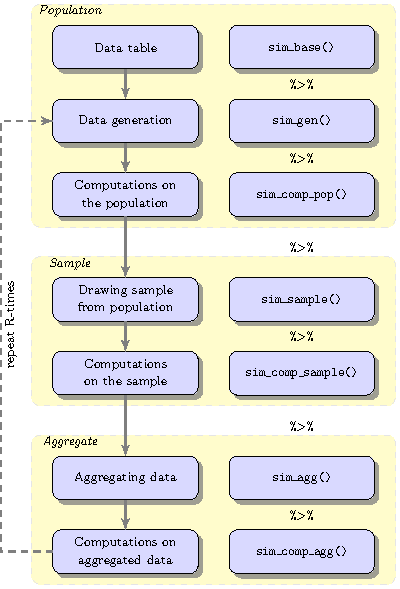
\includegraphics[width=\linewidth]{figs/flowdiagram}

\end{multicols}

%-------------------------------------------------------------------------------
%	Features
%-------------------------------------------------------------------------------

\mysec{Data generation}
%-------------------------------------------------------------------------------

\begin{verse}
\textit{\texttt{saeSim} provides several functions to make the composition and generation of synthetic population data more efficient.}
\end{verse}

\inputR{Rmd/dataGeneration}


\mysec{Outliers}
%-------------------------------------------------------------------------------

\begin{verse}
\textit{Outliers can be added to the data generation. \texttt{sim\_gen\_cont} provides the interface to control the degree and level of contamination.}
\end{verse}

\inputR{Rmd/outliers}
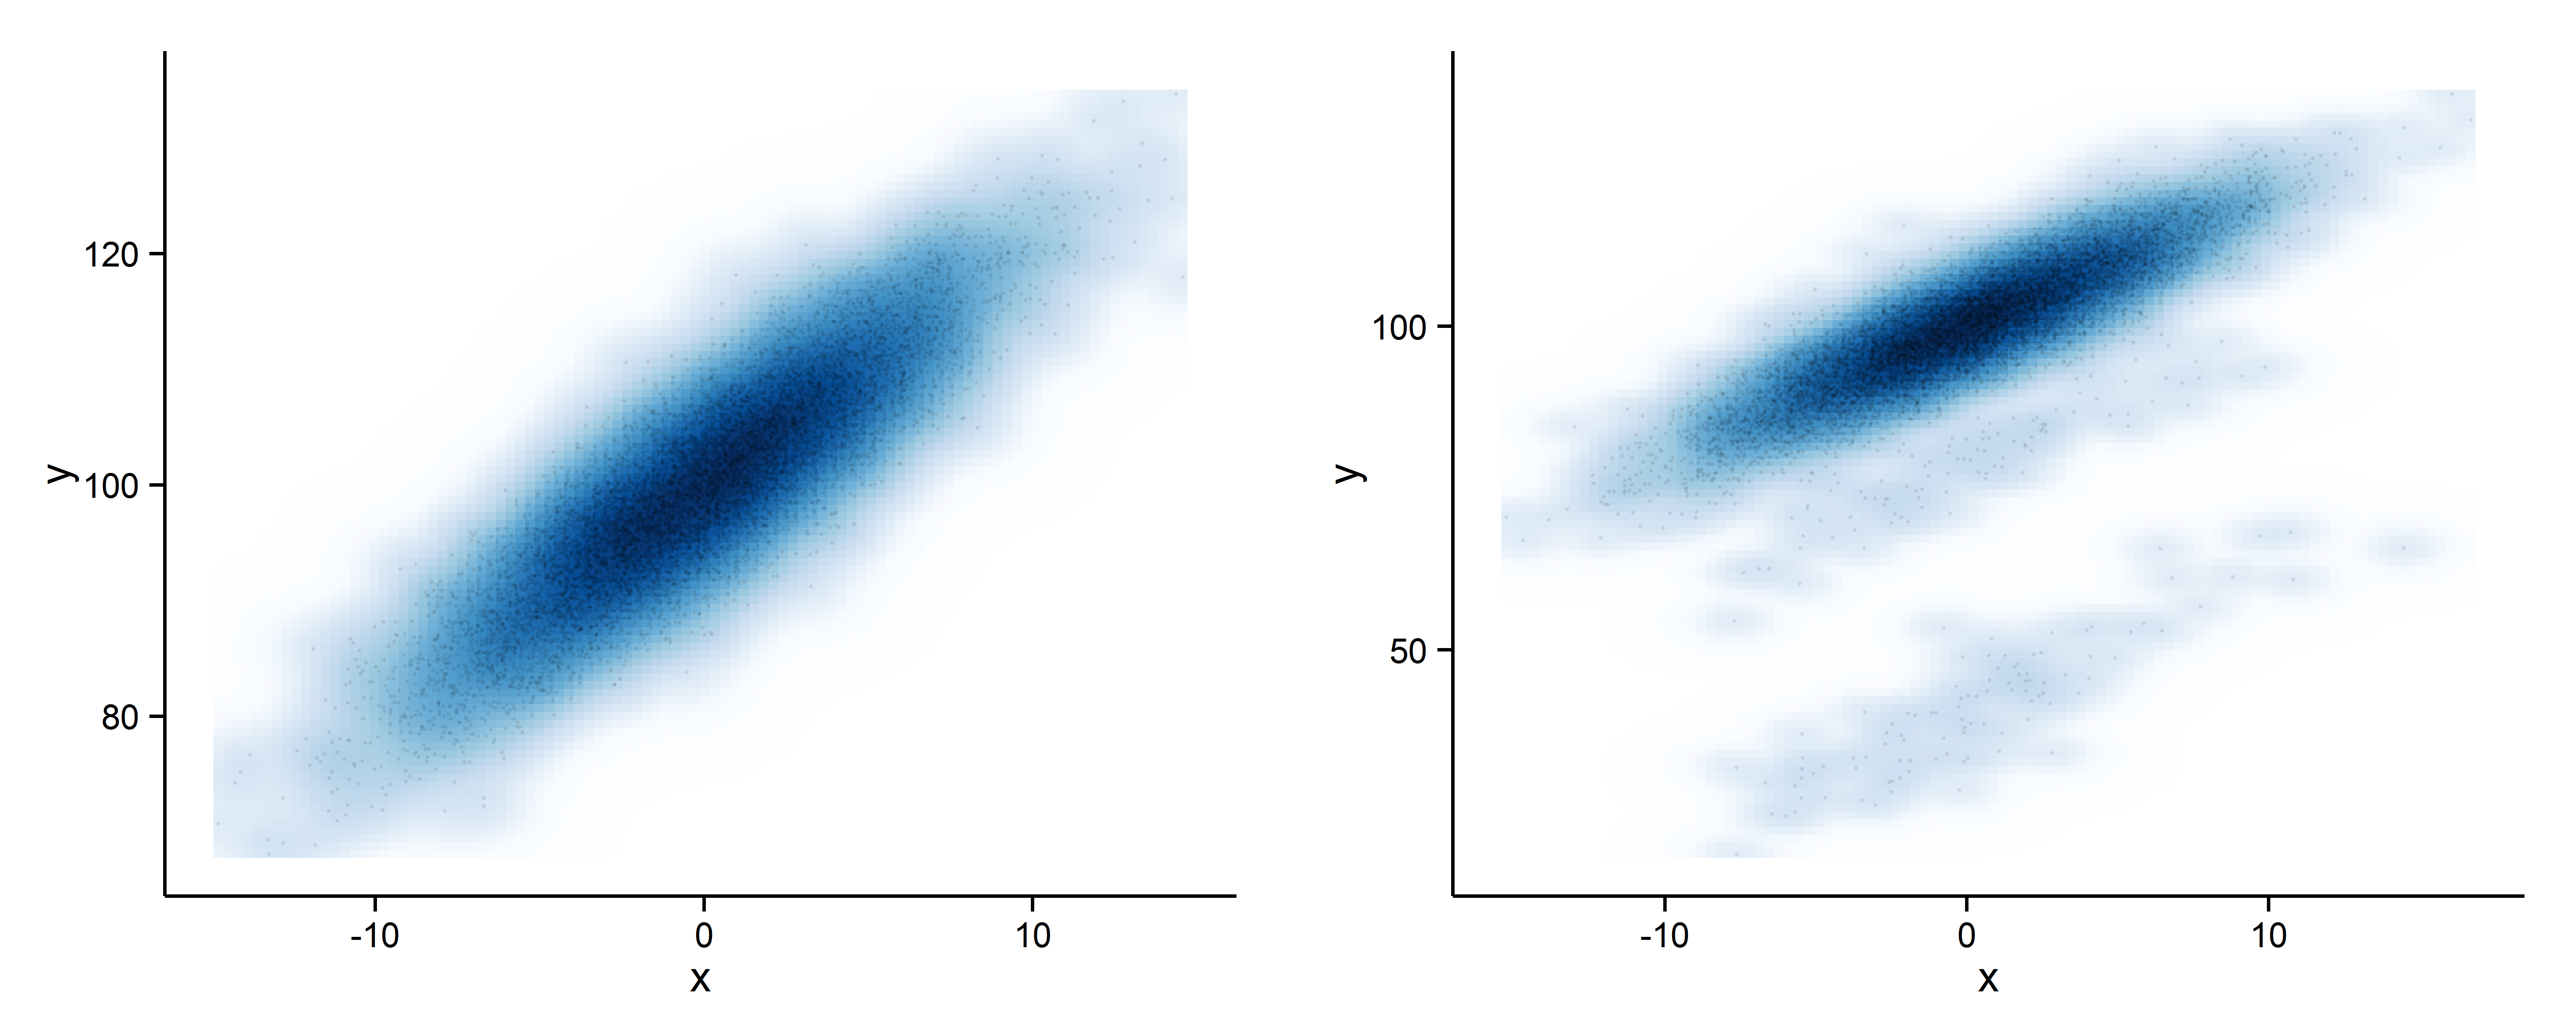
\includegraphics[width=\linewidth]{figs/outliers/outliers-1}

\columnbreak

\mysec{Parallel computations}
%-------------------------------------------------------------------------------

\begin{verse}
\textit{Simulation studies are embarrassingly parallel. For parallel computations we utilize \code{parallelMap} which makes it easy to switch between different parallel back-ends in \code{R}, e.g. multicore, socket, MPI and BatchJobs.}
\end{verse}

\inputR{Rmd/parallelComputations}


\mysec{Extensions}
%-------------------------------------------------------------------------------

\begin{verse}
\textit{To make \texttt{saeSim} more than just a tool for data generation define your own components and arrange them in the process.}
\end{verse}

\begin{itemize}
  \item This is a complete example beginning with data generation, followed by simple random sampling in each domain and completing with a comparison of the mean squared error of the sample mean and the average of a linear predictor in each domain.
  \item Here we define \texttt{comp\_lm} to use a linear model to predict the area means. The data is aggregated for each domain by the aggregation function \texttt{sim\_agg}.
  \item At this time we do not see the need to provide tools for further reshaping and aggregation of results. Instead we rely on existing packages like \texttt{dplyr} which is used after the call to \texttt{sim}.
\end{itemize}

\begin{minipage}[b]{0.55\linewidth}
  \inputR{Rmd/extensions}
\end{minipage}
\hfill
\begin{minipage}[b]{0.45\linewidth}
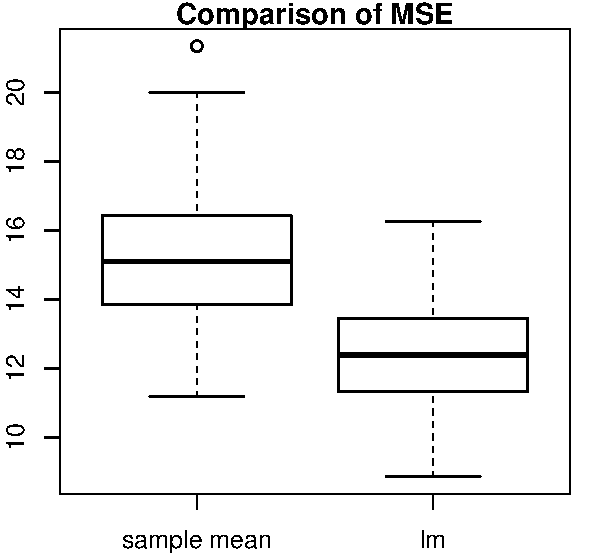
\includegraphics[width=\linewidth]{extensions/extensions_boxplot-1}
\end{minipage}
%----------------------------------------------------------------------------------------
%	CONCLUSIONS
%----------------------------------------------------------------------------------------

\mysec{Design and naming}
%-------------------------------------------------------------------------------

\begin{verse}
\textit{You do not have to redefine, reuse instead!}
\end{verse}
\inputR{Rmd/basicIdea}


\mysec{Remarks}
%-------------------------------------------------------------------------------

\begin{itemize}
  \item We hope to encourage the small area estimation community to contribute and publish the code of simulation studies alongside articles.
  \item \texttt{saeSim} is a suggestion how such studies can be conducted. The design aims to use common tools and to remove control structures from the code. At the same time we encourage the definition of short and self contained functions as \textit{components}.
  \item The package is not complete. If you have suggestions you are welcome to contribute to \texttt{https://github.com/wahani/saeSim}.
\end{itemize}

\color{DarkSlateGray} % Set the color back to DarkSlateGray for the rest of the content

%----------------------------------------------------------------------------------------
%	REFERENCES
%----------------------------------------------------------------------------------------

\nocite{*} % Print all references regardless of whether they were cited in the poster or not
\bibliographystyle{agsm} % Plain referencing style
\bibliography{references} % Use the example bibliography file sample.bib

\end{multicols}

%----------------------------------------------------------------------------------------
%  Author Information
%----------------------------------------------------------------------------------------

\vfill
\vspace{0.5cm}
\begin{minipage}[b]{0.3\linewidth}
  \Large\textbf{Timo Schmid}\\[0.5cm]
  \large 
  Department of Economics\\
  Freie Universit\"at Berlin\\
  \texttt{Timo.Schmid@fu-berlin.de}
\end{minipage}
\hfill
\begin{minipage}[b]{0.3\linewidth}

\includegraphics[width=\linewidth]{FuBerlin}
\end{minipage}
%%
\hfill
%%
\begin{minipage}[b]{0.3\linewidth}
\begin{flushright}
  \Large\textbf{Sebastian Warnholz}\\[0.5cm]
  \large 
  Department of Economics\\
  Freie Universit\"at Berlin\\
  \texttt{Sebastian.Warnholz@fu-berlin.de}
\end{flushright}
\end{minipage}
%

%----------------------------------------------------------------------------------------
\end{document}
%----------------------------------------------------------------------------------------